\chapter{Background}\label{chapter:basics}

Before getting into the details of our driver, some concepts central to any NVMe driver need to be explained in detail first: how communicating with PCIe devices works with Memory-Mapped I/O and Direct Memory Access, the NVMe specification itself, and our programming language of choice, Rust.

\section{PCI Express}
Nowadays, all peripherals, from NVMe SSDs to USB hubs, are connected to the computer via the Periphiral Component Interconnect Express (PCIe) interface. PCIe builds upon PCI and PCI-X defining the specifications of how the computer and peripheral devices interact.

These devices are connected via lanes over the PCIe bus, with transmit and receive channels. For higher throughput, the specification allows for devices with up to 32 lanes, each lane providing a raw bandwidth of \qty[per-mode=symbol]{32}{\giga\bit\per\second} as of PCIe Gen 5.0 \cite{pcie}. PCIe uses a TCP-like protocol for reliable data transmission with features like flow control, congestion avoidance and acknowledgements, with the use of packets.

Configuring PCIe devices is done through accessing the PCI configuration space, depicted by \autoref{fig:pci-config}, a standardized register space containing information and memory addresses of the PCI(e) device. For instance, we can disable interrupts or enable direct memory access (DMA), we configure the ``Command Register'' accordingly.

\begin{figure}[H]
  \centering
    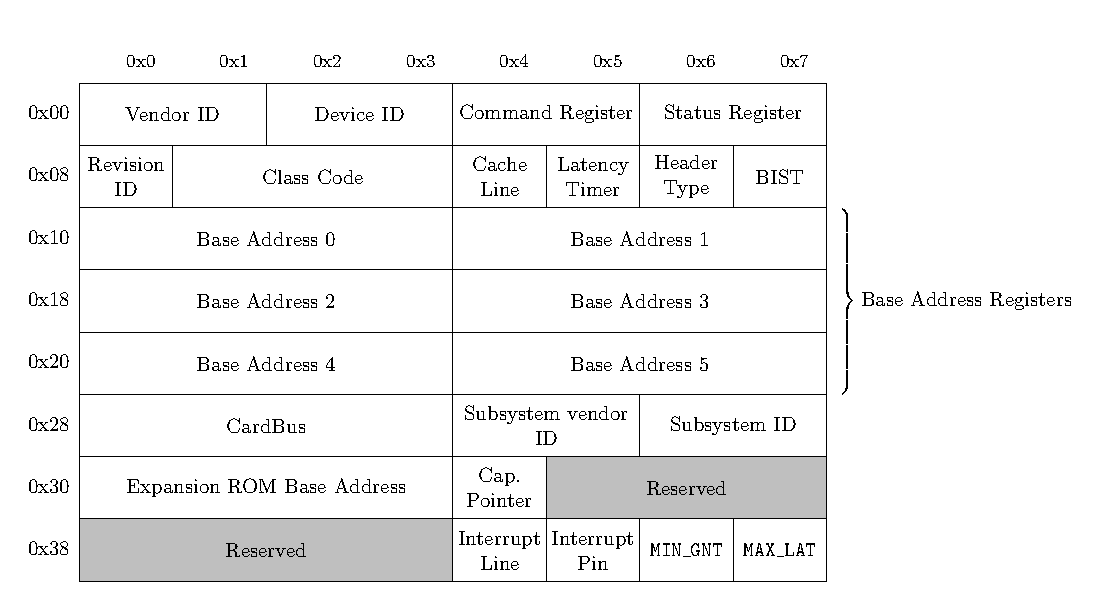
\includegraphics[width=\textwidth]{figures/pcie-config-space}
    \caption{Structure of PCIe configuration space}
    \label{fig:pci-config}
\end{figure}

% \begin{lstlisting}[float,label=lst:sysfs,caption={Example \texttt{sysfs} directory of a PCIe device with domain number 0000, bus number 17 and function 0}]
% /sys/devices/pci0000:17
% |-- 0000:17:00.0
% | \
% |   |-- class
% |   |-- config
% |   |-- device
% |   |-- enable
% |   |-- irq
% |   |-- local_cpus
% |   |-- remove
% |   |-- resource
% |   |-- resource0
% |   |-- resource1
% |   |-- resource2
% |   |-- revision
% |   |-- rom
% |   |-- subsystem_device
% |   |-- subsystem_vendor
% |   |-- vendor
% |-- ...
% \end{lstlisting}


\section{Memory-Mapped I/O}
Memory-mapped I/O (MMIO) is a method of performing I/O operations between the CPU and peripheral devices with a computer. Using MMIO, the memory and register of a PCIe device share the same address space as main memory, allowing these to be addressed the same way as main memory, i.e. using CPU instructions like \texttt{mov}. Historically, peripherals were accessed using port-mapped I/O with specific \texttt{in} and \texttt{out} instructions to access the device's I/O ports via an I/O bus or pins.

The subsystem \texttt{uio} in Linux exposes the device's memory, Base Address Registers (BARs), as well as other required interfaces as files in the pseudo-filesystem \texttt{sysfs}.

\section{Direct Memory Access}
Passing data between hosts and PCIe devices typically is done through the use of direct memory access (DMA); this allows peripheral devices to initiate accesses to main memory independently of the CPU. I/O performance can be improved by not involving the CPU for expensive memory transfers, giving it headroom to perform other operations.

Unlike on older hardware architectures, PCIe does not require a DMA contoller (third-party DMA), rather we can enable ``bus mastering'' (first-party DMA) for PCIe devices; this is required to allow the device to issue memory or I/O requests.

Typically, DMA requires the use of physical addresses, as such bus masters are able to write to any address in main memory. The modern way of performing DMA is to use virtual addresses in conjunction with an input-output memory management unit (IOMMU). Using the IOMMU, DMA operations between a PCIe device and main memory are translated from bus addresses to virtual addresses, which then gets translated to a physical address \cite{spdk-dma}. On Linux, the Virtual Function I/O (VFIO) driver framework enables the use of IOMMU intended for non-privileged, safe user space device drivers \cite{vfio}.


\section{Non-Volatile Memory Express}
Non-Volatile Memory Express (NVMe) itself ``is an open collection of standards and information to fully expose [\ldots] non-volatile memory in all types of computer environments''\footnote{\url{https://nvmexpress.org/about/}}. Relevant for us is the NVMe specification, an open logical device interface specification for accessing non-volatile storage media attached via the PCIe bus. NVMe was designed to capitilise on the low latency and parallelism of SSDs, providing improvements over older storage interfaces such as SATA or SAS in terms of speed and latency. This specification defines several key components:

\begin{itemize}
    \item \textbf{NVMe commands}: the basic units of work that the host system uses to communicate with the NVMe device. These commands may involve I/O operations or administrative tasks. These submission entries contain the command opcode, an identifier, and values pertaining to the command, e.g. data pointers for read/write operations. The structure of such a command can be seen in \autoref{fig:nvme-queue}
    \item \textbf{Submission Queues (SQ)}: The host system places commands here to be processed by the NVMe device. Each NVMe device can support multiple SQs, enabling parallel command processing.
    \item \textbf{Completion Queues (CQ)}: The NVMe device places completion entries noticing that commands have to processed. Each completion queue is associated with a submission queue, however the specification allows multiple submission queues to be associated with a single completion queue.
\end{itemize}

The specification supports 1 Administrative submission and completion queue pair and up to 65535 I/O submission and completion queues, in theory allowing for high scalability and the ability to handle high volumes of I/O requests. Both the submission and completion queue operate as ring buffers, supporting up to 65536 entries and 65535 outstanding requests. Due to the command identifier being 16 bits in size, the NVMe controller in total supports up to 65536 outstanding requests at a time.

Submission and completion queues operate similarly to a Consumer-Producer pattern, e.g. in the case of an SQ, the host produces requests and adds them to the queue for the NVMe device to consume. For the SQ, we keep track of a \texttt{tail} pointer as the producer, pointing to the next free slot and a \texttt{head} pointer, pointing to the next slot to be consumed. For the CQ, we only keep track of the \texttt{head} pointer.

\begin{figure}[]
  \centering
    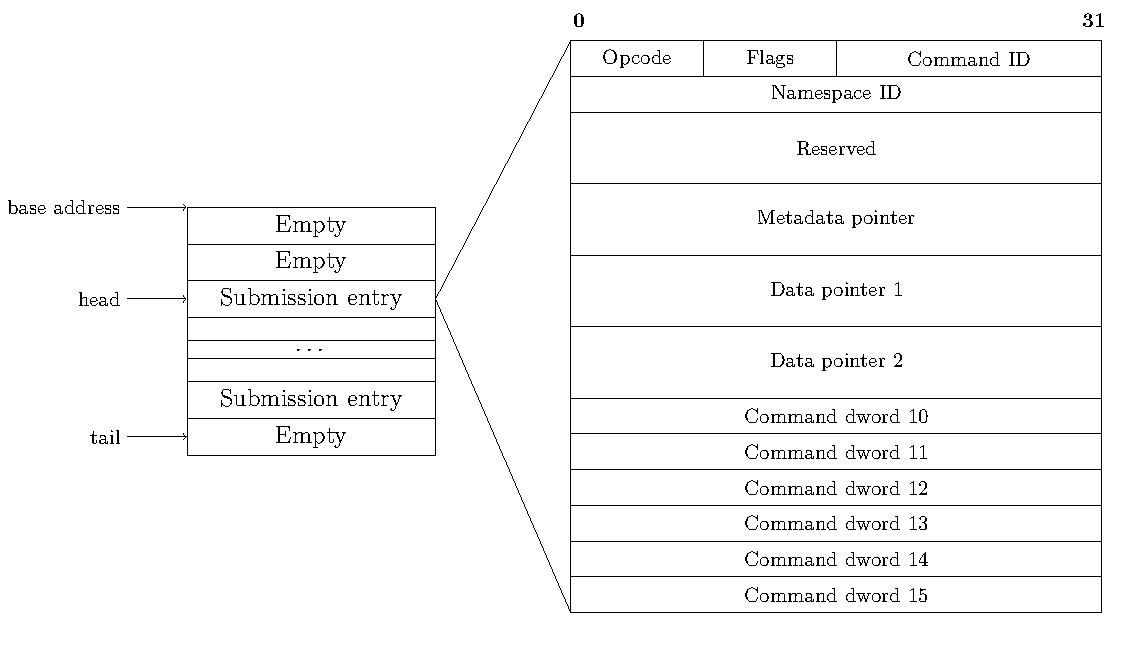
\includegraphics[width=\textwidth]{figures/nvme-queue}
    \caption{Example queue and structure of the NVMe submission entry}
    \label{fig:nvme-queue}
\end{figure}

Submitting requests to the NVMe device is done by constructing and then inserting a submission entry into the queue and updating the corresponding doorbell register to the new \texttt{tail} value, notifying the NVMe device of the newly submitted request. Upon completion, the NVMe controller will post a completion entry into the completion queue belonging to the submission queue. The completion entries contain the command identifier, the status of the operation, and other command specific information. After processing the completion, the host then updates the doorbell register of the completion queue to the new value of \texttt{head} to signal that the completion entry has been acknowledged and processed. Depending on how the driver configures the NVMe controller, the device may send an interrupt signal upon completion.

For reading and writing, depending on the amount of data, different data pointers are passed to the command. The addresses passed to the data pointers are called Physical Region Page (PRP), which is nothing more than a pointer to a physical memory page. There exists another data structure for describing data buffers called Scatter Gather Lists (SGL), however these are not supported by all NVMe SSD's while PRPs are.

\begin{figure}[]
  \centering
    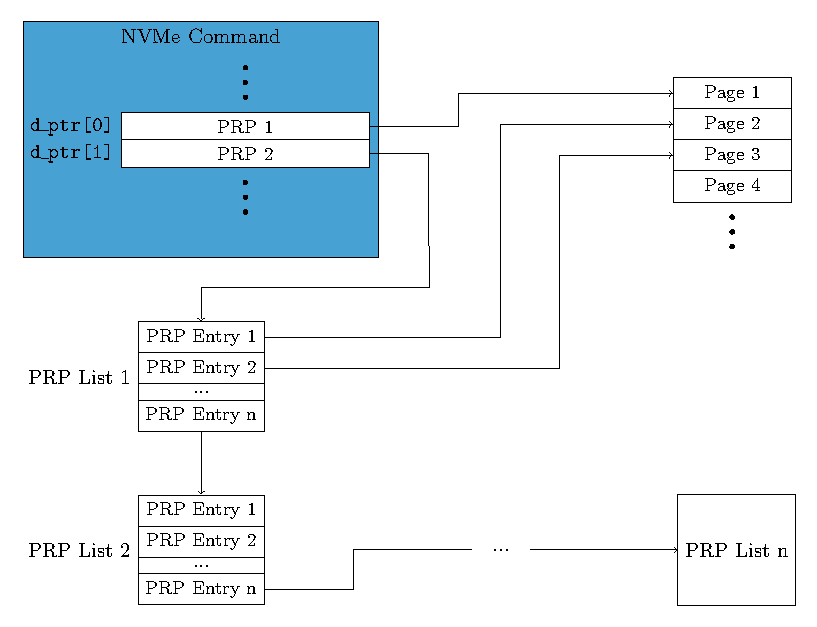
\includegraphics[width=\textwidth]{figures/prp-list}
    \caption{Visualisation of the PRP lists in NVMe commands}
    \label{fig:prp-list}
\end{figure}

For I/O operations sized less or equal to one page (by default 4 KiB) we pass the physical address to Data pointer 1 (\texttt{d\_ptr[0]}). For requests which cross one memory boundary, we set \texttt{d\_ptr[0]} to the physical address and Data pointer 2 (\texttt{d\_ptr[1]}) to the address of the second block of data, e.g. \texttt{d\_ptr[0] + nvme\_page\_size} for contiguous memory. Once the I/O operation spans more than two pages, a pointer to a PRP list is passed to \texttt{d\_ptr[1]}; this is depicted in \autoref{fig:prp-list}. A PRP list is a list of PRP entries, where the last entry points to the next PRP list; essentially an array of pointers.

\section{Rust}
Memory bugs remain amongst the most exploited vulnerabilities \cite{mitre}, and companies such as Google have begun to transition away from C and C++ towards the use of memory-safe languages, like Java, Rust or Go \cite{google}. Meanwhile, there exists an effort to integrate Rust into the Linux kernel spearheaded by the Rust for Linux project\footnote{\url{https://rust-for-linux.com/}}, with Linux adopting support for the programming language with release 6.1.

Rust\footnote{\url{https://www.rust-lang.org/}} is a modern systems programming language with a focus on safety, speed and concurrency. It was designed to provide memory and thread safety guarantees through a unique onwership model without any performance pitfalls. These safety checks are done at compile time, eliminating common bugs like null-pointer dereferences and data races. Furthermore, Rust is a compiled language without a garbage collector, leading to much better performance compared to interpreted languages and less overhead compared to languages that have a garbage collector.

With all these factors in mind, Rust seems to be an ideal programming language for developing (user space) device drivers where safety and effiency are paramount.

% \begin{lstlisting}[float,language=Rust,label=lst:nvme_command,caption=NVMe command defined as a struct in Rust]
% #[repr(packed)]
% pub struct NvmeCommand {
%     pub opcode: u8,        // Command opcode
%     pub flags: u8,
%     pub c_id: u16,         // Command ID
%     pub ns_id: u32,        // Namespace ID
%     pub _rsvd: u64,        // Reserved
%     pub md_ptr: u64,       // Metadata pointer
%     pub d_ptr: [u64; 2],   // Data pointers
%     pub cdw10: u32,        // Command dwords; usage is command specific
%     pub cdw11: u32,
%     pub cdw12: u32,
%     pub cdw13: u32,
%     pub cdw14: u32,
%     pub cdw15: u32,
% } // 64 bytes
% \end{lstlisting}

% \begin{lstlisting}[float,language=Rust,label=lst:nvme_completion,caption=NVMe completion entry defined as a struct in Rust]
% #[repr(packed)]
% pub struct NvmeCompletion {
%     pub command_specific: u32,
%     pub _rsvd: u32, // Reserved
%     pub sq_head: u16, // Submission Queue head
%     pub sq_id: u16, // Submission Queue ID
%     pub c_id: u16, // Command ID
%     pub status: u16, // Status field
% } // 16 bytes
% \end{lstlisting}
